\documentclass{report}
\usepackage[margin=1in, paperwidth=8.5in, paperheight=11in]{geometry}
%Math packages%
\usepackage{amsmath}
\usepackage{amsthm}
%Spacing%
\usepackage{setspace}
\onehalfspacing
%Lecture number%
\newcommand{\lectureNum}{14}
%Variables - Date and Course%
\newcommand{\curDate}{February 16, 2017}
\newcommand{\course}{CS 241}
\newcommand{\instructor}{Kevin Lanctot}
%Defining the example tag%
%\theoremstyle{definition}%
\newtheorem{ex}{Example}[section]
%Setting counter given the lecture number%
\setcounter{chapter}{\lectureNum{}}
%Package to insert code%
\usepackage{listings}
\usepackage{courier}
\usepackage{xcolor}
\lstset { %
    tabsize=2,
    breaklines=true,
    language=C++,
    backgroundcolor=\color{blue!8}, % set backgroundcolor
    basicstyle=\footnotesize\ttfamily,% basic font setting
}
%Package for images%
\usepackage{graphicx}

\begin{document}
%Note title%
\begin{center}
\begin{Large}
\textsc{\course{} | Lecture \lectureNum{}}
\end{Large}
\end{center} 
\noindent \textit{Bartosz Antczak} \hfill
\textit{Instructor: \instructor{}} \hfill
\textit{\curDate{}}
\rule{\textwidth}{0.4pt}
% Actual Notes%
\subsubsection{Recall | Ambiguous Grammar}
Since grammar can be ambiguous (i.e., "$9 + 3 / 3 = 4 \,\mathrm{or} \, 10?$), we can have multiple parse trees for the same expression. The resulting string from a parse tree depends on how we \textit{traverse} it. To make it unambiguous, we need to have a more formal set of production rules:
\begin{itemize}
\item $\alpha A \beta$ \textit{directly derives} $\alpha \gamma \beta$ if there is a production rule $A \rightarrow \gamma$, where:
\begin{itemize}
\item $A \in N$ (non-terminals), and
\item $\alpha, \beta, \gamma \in (N \cup T)$ (non-terminals, terminals, empty string)
\end{itemize}
Informally, ``directly derives" means it takes one derivation step or one application of a production rule.
\item $\alpha A \beta$ \textit{derives} $\alpha \gamma \beta$ if there is a finite sequence of productions $\alpha A \beta \rightarrow \alpha \Theta_1 \beta \rightarrow \alpha \Theta_2 \beta \rightarrow \cdots \rightarrow \alpha \gamma \beta$, where again:
\begin{itemize}
\item $A \in N$ (non-terminals), and
\item $\alpha, \beta, \gamma \in (N \cup T)$ (non-terminals, terminals, empty string)
\end{itemize}
It is written as $\alpha A \beta \implies^* \alpha \gamma \beta$
\end{itemize}
To reduce ambiguity, we will set up some standard for reading strings:
\begin{itemize}
\item \textbf{Associativity:} how we evaluate symbols (e.g., $6 - 3 + 4$: do we read it as $(6-3)+4$ or $6 - (3+4)$?). We will set a standard for \textit{left associativity}
\item \textbf{Precedence:} grouping non-equivalent terminals. For instance, in arithmetic, multiplication takes precedence over addition.
\end{itemize}
\section{Top-Down Parsing}
\textbf{Parsing} is the approach to determining if a certain string is valid in a given grammar. In other words, given a grammar $G$ and a word $w$, \textit{find a derivation for w}.\\
Our goal in this section is to look at the characters in $w$ and decide which rules derived $w$ from the start symbol.
\subsection{Approach 1 | Backtracking}
We can use a \textit{backtracking algorithm} for parsing, which considers every possible derivation and stops once it finds a valid one. This approach is very exhaustive, so let's try another approach.
\subsection{Approach 2 | Stack-based Parsing}
Use a stack to remember information about our derivations and/or processed input. To use stack-based parsing, we must also \textit{augment} our grammar by adding a two new characters: one to mark the beginning of a word (called BOF) and one to mark the end of a word (called EOF). We must also define a new start symbol $S^\prime$ that only appears once as $S \rightarrow start S end$
%TODO look for start + end symbols%
.The method works like this:
\begin{itemize}
\item Start by pushing $S^\prime$ on to the stack
\item For every item on top of the stack:
\begin{itemize}
\item If it is a \textbf{non-terminal}, expand it using a production rule where the resulting string matches the input
\item If it is a \textbf{terminal}, match it with the input. Pop the terminal off the stack and read the next character from the input
\end{itemize}
\end{itemize}
If you try to pop when the stack is empty, or when the stack is not empty when you are finished processing, that results in an ERROR.
\begin{ex}
The first few steps in deriving ``abywz" from a given grammar (the remaining steps follow the same procedure as the first few steps and were omitted to save space)
\end{ex}
\begin{figure}[ht]
\begin{center}
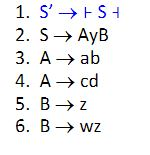
\includegraphics[scale=0.7]{rules1.jpg}
\end{center}
\caption{The production rules for this particular grammar example. Courtesy of Prof. Lanctot's slides.}
\end{figure}
\begin{figure}[ht]
\begin{center}
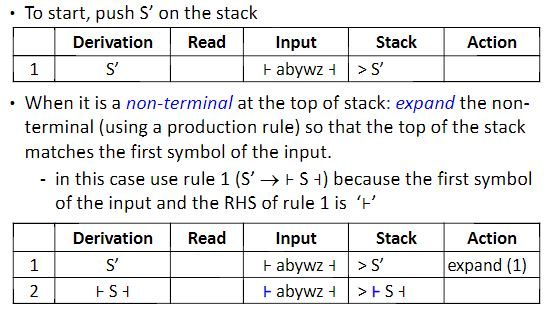
\includegraphics[scale=0.5]{ex1_1.jpg}
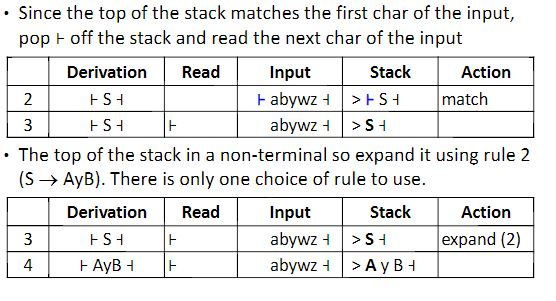
\includegraphics[scale=0.5]{ex1_2.jpg}
\end{center}
\caption{The stack approach. Courtesy of Prof. Lanctot's slides.}
\end{figure}
Now that we know how this works, one problem still stands: how are we able to correctly predict which rule applies? 
\subsection{LL(1) Parsing}
LL(1) parsing is named after:
\begin{itemize}
\item Processing the input from \textbf{L}eft to right, finding a \textbf{L}eftmost derivation, and the algorithm allows us to look ahead \textbf{1} token.
\end{itemize}
For all LL(1) grammars, given an $A$ on the top of the stack and an $a$ as the next input character, at most one rule can apply. These restrictions cause our reading to be unambiguous. We do this by constructing a \textit{predictor table}.
\begin{figure}[ht]
\begin{center}
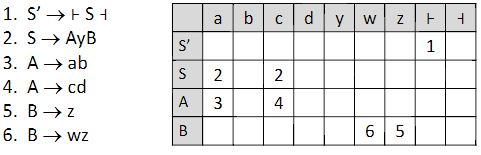
\includegraphics[scale=0.9]{predict.jpg}
\end{center}
\caption{A sample predictor table. Courtesy of Prof. Lanctot's slides.}
\end{figure}
\subsubsection{Constructing a Predictor Table}
To build a method \texttt{predict(A, a)}, we require two helper methods. The method \texttt{predict(A, a)} outputs maps the input values to their respective value in the predictor table. The two helper methods are:
\begin{itemize}
\item \texttt{follow(A)}: this method answers the question, \textit{starting from the start symbol, does the terminal b ever occur immediately following A?} Here, $b \in T, A \in N$
\item \texttt{empty($\alpha$)}: answers the question, \textit{can $\alpha$ disappear?} This method returns true if $\alpha \rightarrow^* \varepsilon$. It returns false if $\alpha$ has a terminal in it
\end{itemize}
With these helper methods, we can calculate \texttt{predict(A, a)}. Here, we're asking \textit{if A is on the top of the stack and a is the next symbol in the input, which rule should be used to expand A?}.
%END%
\end{document}